\chapter{Vaatimukset ja järjestelmän kuvaus} % Itse luvun otsikko. Huom ei numeroa!                                         santeri on ruma
\label{kuvaus} % Tähän kappaleeseen voi viitata \ref{kuvaus}
\thispagestyle{fancy} % Tarvitaan, jotta header/footer näkyvät otsikkosivuilla


\section{Mallintaminen}  % 3.1
    Tässä kappaleessa kuvaillaan käyttäjätarinoita ja havainnollistetaan niihin liittyviä toimintoja. 

\subsection{Kayttotapauskaavio(t)}    % 3.1.1

\subsubsection{Käyttäjätapaus 1: Käyttäjätietojen tarkastelu}   % 3.1.1.1

    Antti Asiakas haluaa tarkastella itseään koskevia tietoja sekä raportteja. Antin tulee valita etusivulta löytyvä
    \textit{Omat tiedot} -painike, jotta hän pääsee katsomaan omia tietojaan. Toimintoja on havainnollistettu kuvassa \ref{img:kayttotapaus1}, sivulla \pageref{img:kayttotapaus1}.

    Täältä Antti voi esimerkiksi:

    \begin{itemize}
        \item tarkastella ja muuttaa omia yhteystietojaan
        \item tarkastella itseään koskevia raportteja
        \item poistaa itsensä järjestelmästä
        \item kirjautua ulos
    \end{itemize}

    Jos Antti valitsee itseään koskevat raportit, järjestelmä esittää hänelle hänen oman ostohistoriansa,
    voimassa olevat alennukset sekä mahdolliset suurostobonukset.
    Mikäli Antilla ei ole aiempaa historiaa Megantin kanssa, järjestelmä ei tarjoa hänelle raporttia.

    \begin{figure}[H]
        \centering
        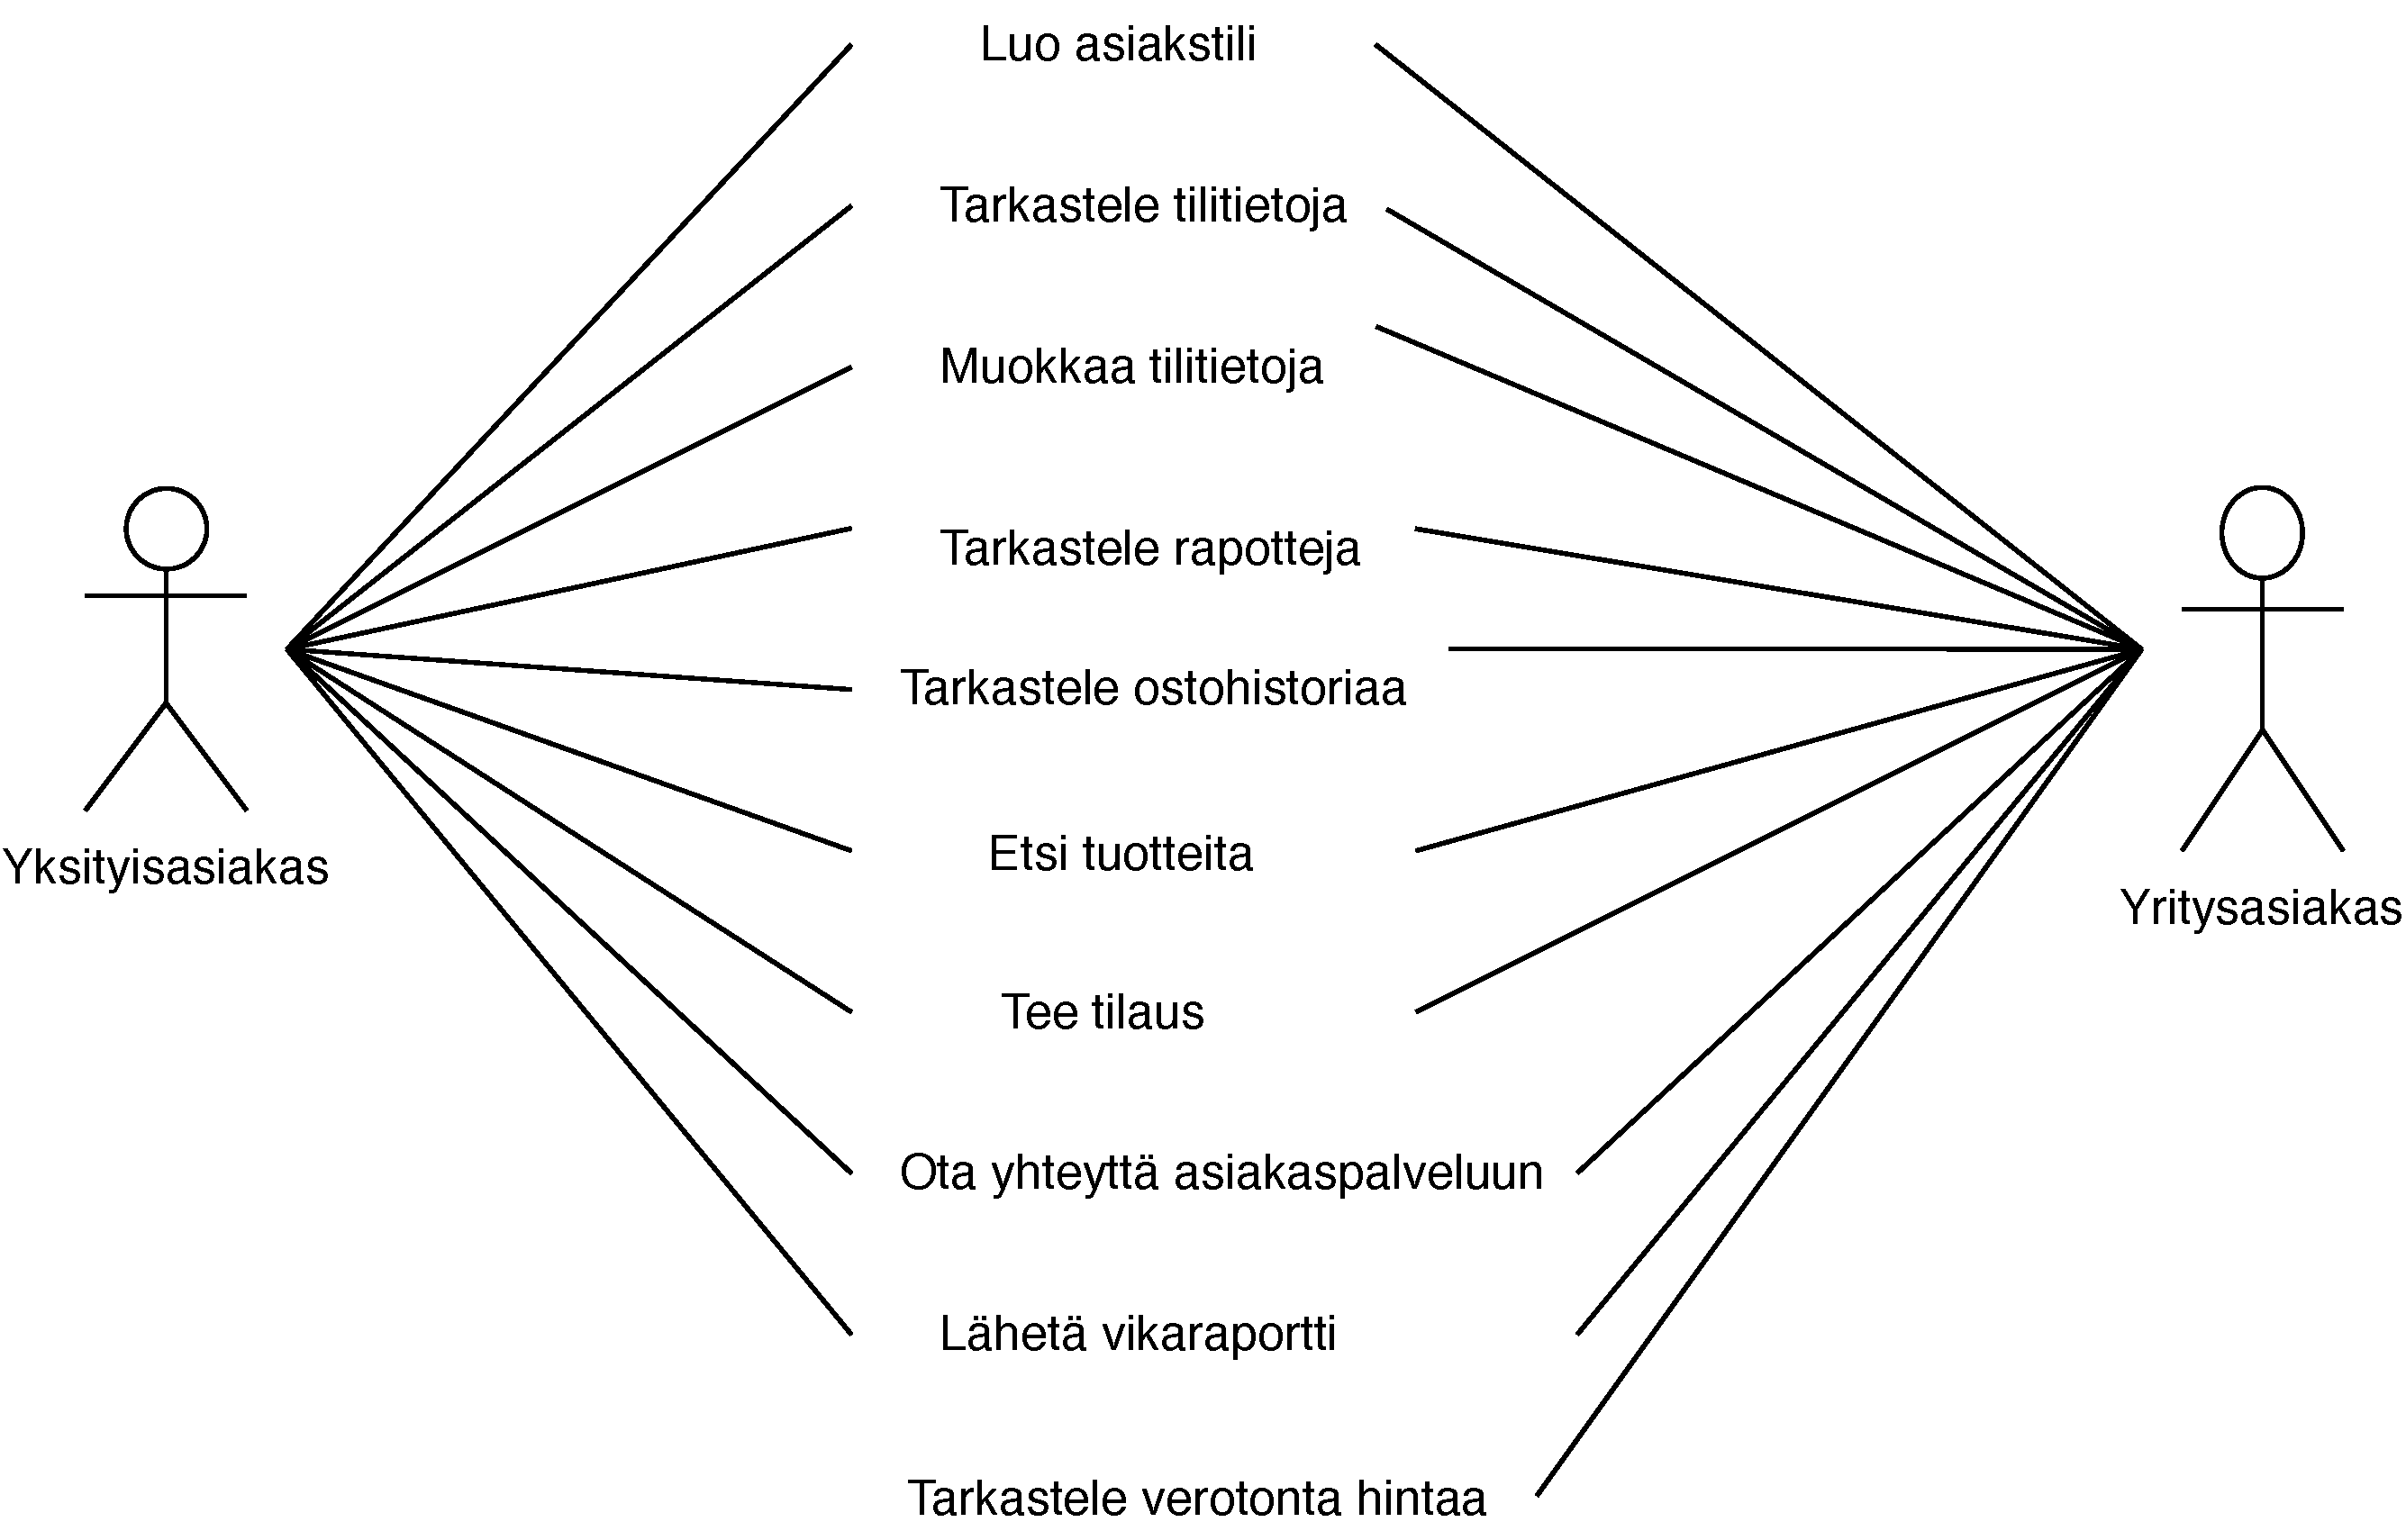
\includegraphics[width=0.85\textwidth]{kayttotapauskaavio1.pdf}
        \caption{Käyttötapauskaavio asiakkaan näkökulmasta}
        \label{img:kayttotapaus1}
    \end{figure}

    Sisäisiin käyttäjiin lukeutuvat kaikki yrityksen sisäiset toimijat. Sisäisten käyttäjien käyttötapauskaavio on liitteessä \ref{kayttotapaus2}. 

\subsubsection{Käyttäjätapaus 2: Personoidun tarjouksen/tarjouksien luonti ja lähet\-täminen}     % 3.1.1.2

    Järjestelmä ehdottaa Mikko Myyntitykille mahdollista alennusta koskien tiettyä asiakasryhmää.
    Mahdollinen alennus perustuu järjestelmän omiin sisäisiin statistiikkoihin ja algoritmeihin.
    Mikko voi hyväksyä, olla hyväksymättä alennusta, tai halutessaan määritellä tarjouksen itse.
    Jos Mikko syöttää järjestelmään alennuksen, joka on erittäin suuri, järjestelmä antaa hänelle varoituksen.
    Mikko voi myös tarkastaa, että järjestelmä ei luo alennuksia, jotka ovat liian suuria tai pieniä.
    Alennusta myönnettäessä määritellään sen suuruus, kesto, tuoteryhmät sekä asiakaskohderyhmä.

    Jos jonkinlainen alennus myönnetään, järjestelmä lähettää asiakasryhmälle sähköisen ilmoituksen alennuksesta (tarjouskirje).

\subsection{Tietoyhteyskaavio}   % 3.1.2

    Järjestelmän rakennetta koskeva tietoyhteyskaavio esitellään kuvassa \ref{img:tietoyhteyskaavio}, sivulla \pageref{img:tietoyhteyskaavio}.

    \begin{figure}[h]
        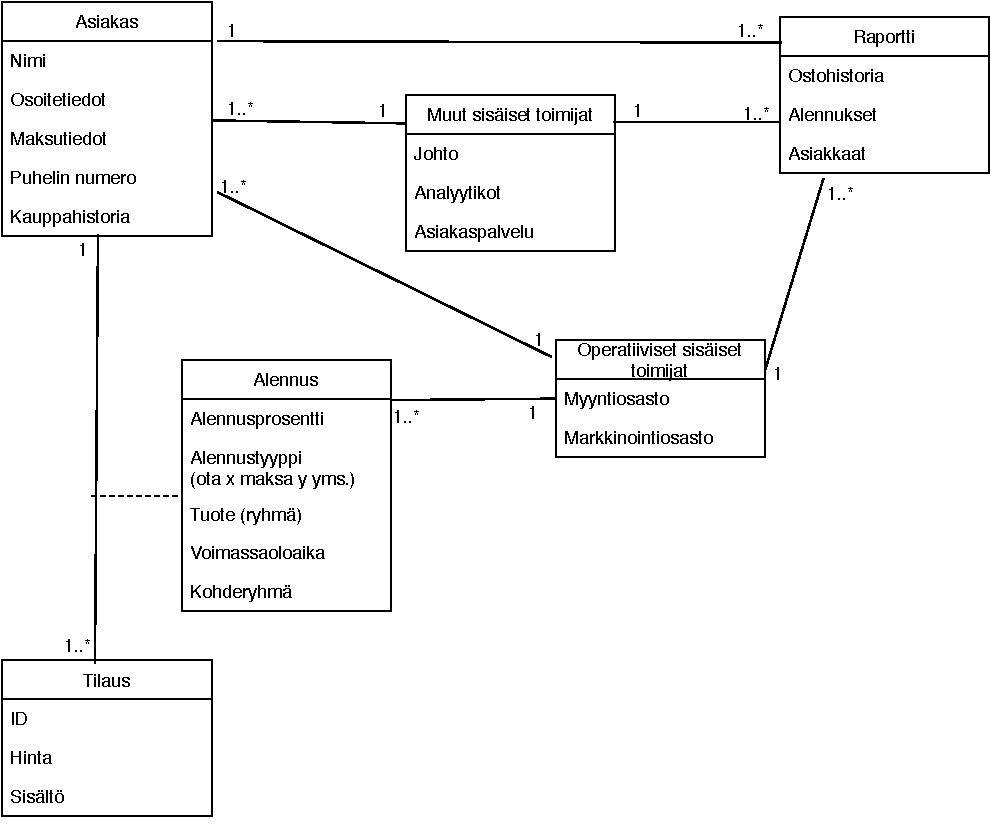
\includegraphics[width=\textwidth]{Tietoyhteyskaavio.pdf}
        \caption{Tietoyhteyskaavio Megantin CRM:lle}
        \label{img:tietoyhteyskaavio}
    \end{figure}

    \pagebreak

\subsection{Navigointikaavio}     % 3.1.3
    
    Esimerkit asiakkaan navigointikaaviosta on kuvassa \ref{img:nkasiakas}, sivulla \pageref{img:nkasiakas}. Asiakas voi muunmuassa muokata omia tietojaan, tarkastella tilauksiaan ja tilata raportin omista tiedoistaan.

    \begin{figure}[h]
        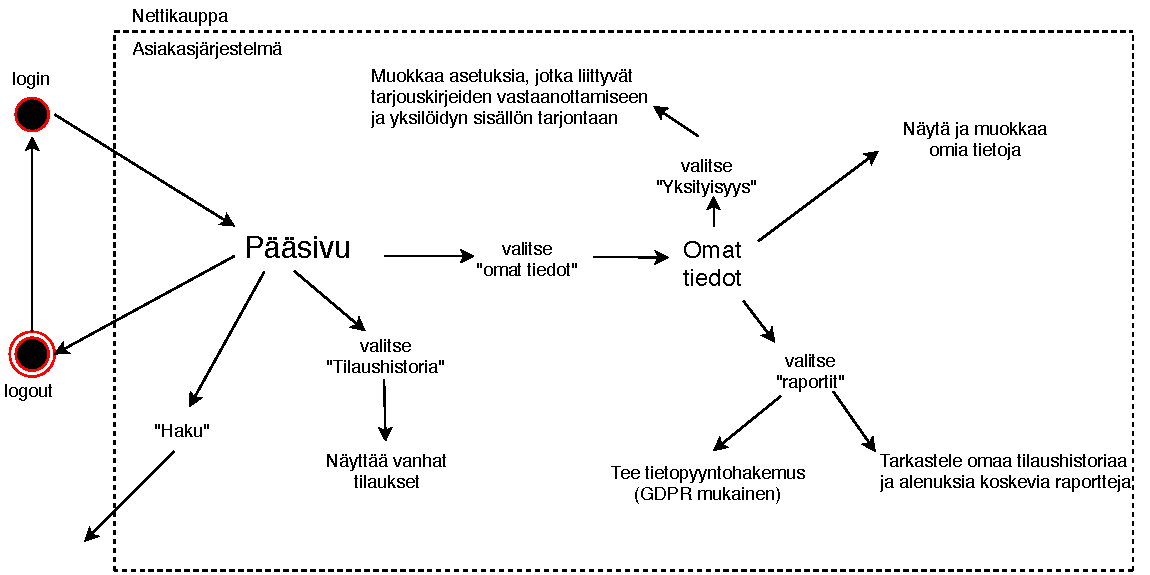
\includegraphics[width=\textwidth]{nkasiakas.pdf}
        \caption{Asiakkaan navigointikaavio}
        \label{img:nkasiakas}
    \end{figure}
    
    Sisäisen toimijan navigointikaaviota on kuvattu myyjän perspektiivistä kuvassa \ref{img:nkmyyja}, sivulla \pageref{img:nkmyyja}. Myyjällä on esimerkiksi oikeudet tarkastella kaikkien asiakkaiden tietoja ja tilauksia, sekä luoda ja lähettää heille tarjouksia (alennukset).
    Hän voi myös tarkastella erilaisia raportteja, jotka voivat olla automaattisesti luotuja tai analyytikoiden tuottamia.
    
    \begin{figure}[h]
        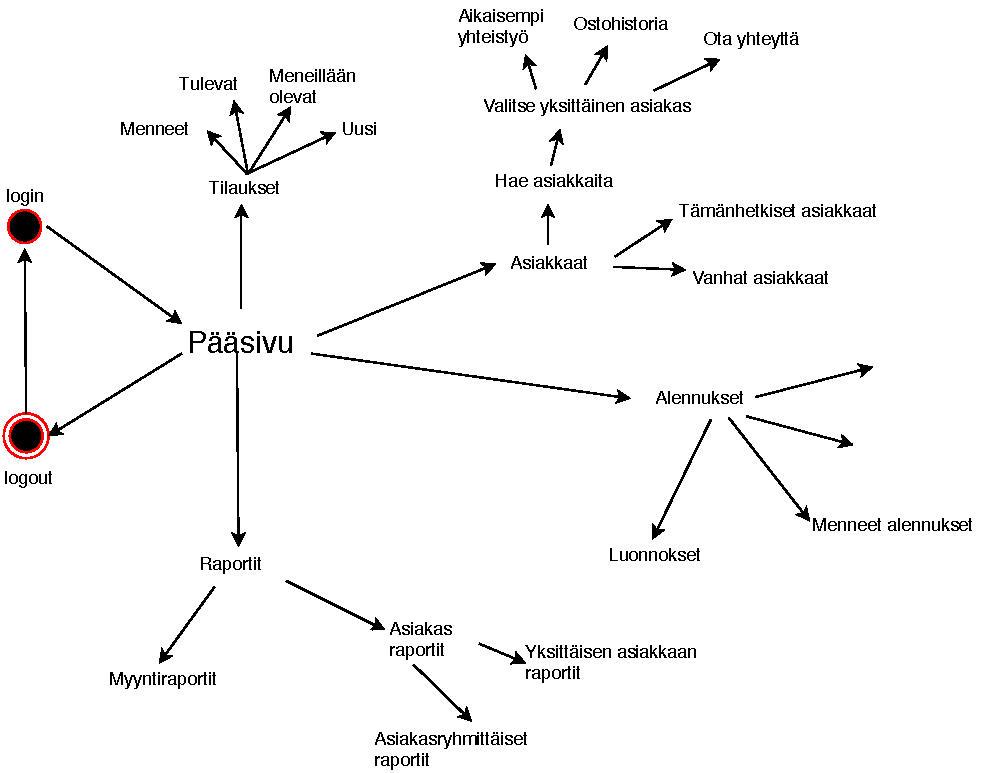
\includegraphics[width=\textwidth]{nkmyyja.pdf}
        \caption{Myyjän navigointikaavio}
        \label{img:nkmyyja}
    \end{figure}

    \pagebreak

\section{Käyttöliittymä}  % 3.2
    
    Kaikki järjestelmän käyttöliittymää kuvaavat esimerkit ovat liitteessä \ref{kayttoliittyma}. Näkymiä ovat asiakkaan näkymä, sisäisen käyttäjän pää- ja työnäkymät, sekä ylläpidon näkymä.
    
    Esimerkkinä käyttöliittymästä käyttäjän päänäkymä kuvassa \ref{img:asiakasesimerkki}, sivulla \pageref{img:asiakasesimerkki}.

    \begin{figure}[h!]
        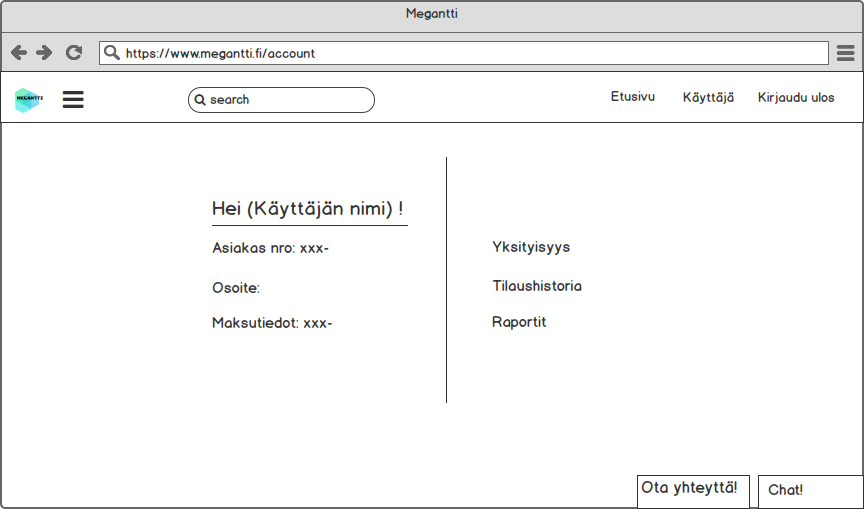
\includegraphics[width=\textwidth]{gui/asiakas.png}
        \caption{Asiakkaan päänäkymä}
        \label{img:asiakasesimerkki}
    \end{figure}

\section{Vaatimukset}       % 3.3

    Tässä kappaleessa esitellään järjestelmää koskevia lopullisia vaatimuksia, jotka ovat taulukoituna liitteessä \ref{tab:vaatimukset2}.
    Lisäksi syvennytään paremmin kahteen vaatimukseen, joista toinen on toiminnallinen, ja toinen ei-toiminnallinen
    vaatimus.

    \subsection{Esimerkkivaatimus 1: Loki}
        % Tarkempi kuvaus toiminnallisesta vaatimuksesta, joka ei ole suoraan sidoksissa käyttäjän tekemisiin (esim joku automaattitoiminnoista)
        Järjestelmän tulee pitää kirjaa järjestelmätapahtumista. Tämä sisältää kaikki muutokset mitä eri käyttäjät (niin sisäiset kuin ulkoisetkin) tekevät.
        Se sisältää tiedot myös kaikista ostoksista, tilinsiirroista ja alennuksista. Osa näistä tiedoista poistetaan välimuistista tietyn ajan 
        jälkeen. Tällaisia tietoja ovat esimerkiksi käyttähän osoitetietojen muutokset. Järjestelmän ylläpitäjät voivat käyttää tätä dataa hyödyksi tarkastellessaan 
        järjestelmän tilaa. 
    \subsection{Esimerkkivaatimus 2: Access Policy}
        % Tarkempi kuvaus ei-toiminnallisesta vaatimuksesta
        Järjestelmässä tulee olla selkeä \textit{Access policy} käyttäjille. Tämä tullaan käytännössä toteuttamaan
        minumum access policy -periaatetta, eli jokaisella käyttäjällä on minimioikeudet järjestelmään.
        Tämä käytäntö suojaa sekä yksittäistä laitetta, että koko verkkoa, jossa järjestelmä on käytössä. 
        \cite{kurssi, sommerville}

\section{Ympäristö}     % 3.4

    Seuraavissa kappaleissa käsitellään järjestelmän ympäristöä. Ympäristöllä takoitettaan muita järjestelmiä tai toimintoja, joiden kanssa uusi \gls{crm} tulee olemaan tekemisissä joko suoraan tai epäsuorasti.
    
    Ympäristöön luetaan myös ohjelmistoon epäsuorasti vaikuttavat tekijät mm. virransyöttö ja laitearkkitehtuuri.
    \cite{sommerville}

    \subsection{Liittyvät järjestelmät}     % 3.4.1
        % Mitä liittyviä järjestelmiä on (esim vanha järjestelmä, viranomaisjärjestelmät, muut yrityksen järjestelmät)? Mitä vaatimuksia ne asettavat määrittelydokumentin järjestelmälle?
        Uusi \gls{crm} tulee käytännössä integroitumaan jo olemassa olevan \gls{erp} järjestelmän alijärjestelmäksi. Näinollen sen tulee pystyä kommunikoimaan
         muunmuassa olemassaolevan tietokannan kanssa. Kommunikointiin kuuluu muunmuassa tilausten, asiakastietojen, tuotteiden ja myyntihistorian hakeminen, 
         luominen, ja muuttaminen järjestelmässä. Uudella \gls{crm}:llä ei tule olemaan omaa tietokantaa, vaan se hyödyntää jo olemassaolevaa tietokantaa suoraan. 
         \cite{erp, crm2}

    \subsection{Tarvittavat yhteydet ja muut ympäristön vaatimukset}  % 3.4.2
        % Ympäristön (toiminta-tai käyttöympäristö) asettamia vaatimuksia? Mitä vaaditaan järjestelmältä, mitä järjestelmä vaatii ympäristöltä.
        Koska \gls{crm} tulee käyttämään jo olemassaolevan \gls{erp}:n tietokantaa, tulee se sijoittaa fyysisesti mahdollisimman lähelle tietokantapalvelun
        tarjoavaa järjestelmää. Näin saadaan minimoitua mahdollinen latenssi järjestelmien välillä ja nopeutettua operaatioiden suoritusta. Suositusnopeus 
        \gls{crm}:n ja \gls{erp}:n välillä käytettävälle linkille on 40Gbit/s ja sen tulisi olla kahdennettu (\gls{redundantg}). \cite{crm}

        Järjestelmän saatavuus tulisi myös taata replikoimalla palvelimia vähintään kolmeen instanssiin. Tämä voidaan käytännössä toteuttaa esimerkiksi virtualisoinnin 
        (\gls{virtualg}) avulla. Näin saatavuus säilyy vaikka yhdessä instanssissa ilmenisikin ongelma. 
        
        Järjestelmän virransyöttö tulee hoitaa kokonaan \gls{ups} kautta. Näin turvaudutaan mahdollisilta virtapiikeiltä ja/tai häiriötilanteilta ja järjestelmä saadaan
        sammutettua hallitusti myös ulkoisen virransyötön katketessa. 
        
        Koska järjestelmään pääsee käsiksi myös internetin kautta, tulee sille tarjota mahdollisimman nopea linkki internetiin. Tämän linkin suositusnopeus on minimissään 
        1Gbit/s molempiin suuntiin (palvelimelta internetiin ja toisinpäin). 
        Palvelintila tulisi olla sellainen, johon vain kyseiseen tilaan kulkuluvan omaavilla on pääsy. Tällainen kulkulupa tulisi olla minimimäärällä henkilöstöä, mitä mahdollista. 

\section{Jatkokehitysajatukset}     % 3.5

    Vaikka järjestelmä on tarkoitettu nykyisellä rakenteella Megantti konsernin käyttöön, niin sitä on kuitenkin tulevaisuudessa
    mahdollisuus jatkokehittää ja tuotteistaa, jolloin Megantti voisi tarjota sitä muille yrityksille valmiina CRM:änä.

    Myös, jos Megantti laajentaa toimintaa kansainvälisille markkinoille ja näille tytäryhtiöille otetaan myös käyttöön rakennettava
    CMR, tulee vähintään järjestelmän kieliä lisätä. Todennäköisesti myös uusia rajapintajärjestelmiä tulisi ottaa huomioon ja implementoida.

\section{Avoimet asiat}     % 3.6

    Tässä vaiheessa projektia ei ole ilmeentyt avoimia asioita, joita pitäisi erityisesti huomioida. Kuitenkin on todennäköistä, että toteutuksen aikana niitä kuitenkin
    ilmenee, vaikka valmistautuminen ja määrittely olisi tehty kuinka hyvin tahansa.




   
